% Options for packages loaded elsewhere
\PassOptionsToPackage{unicode}{hyperref}
\PassOptionsToPackage{hyphens}{url}
%
\documentclass[
  12pt,
]{article}
\usepackage{amsmath,amssymb}
\usepackage{iftex}
\ifPDFTeX
  \usepackage[T1]{fontenc}
  \usepackage[utf8]{inputenc}
  \usepackage{textcomp} % provide euro and other symbols
\else % if luatex or xetex
  \usepackage{unicode-math} % this also loads fontspec
  \defaultfontfeatures{Scale=MatchLowercase}
  \defaultfontfeatures[\rmfamily]{Ligatures=TeX,Scale=1}
\fi
\usepackage{lmodern}
\ifPDFTeX\else
  % xetex/luatex font selection
    \setmainfont[]{Times New Roman}
\fi
% Use upquote if available, for straight quotes in verbatim environments
\IfFileExists{upquote.sty}{\usepackage{upquote}}{}
\IfFileExists{microtype.sty}{% use microtype if available
  \usepackage[]{microtype}
  \UseMicrotypeSet[protrusion]{basicmath} % disable protrusion for tt fonts
}{}
\makeatletter
\@ifundefined{KOMAClassName}{% if non-KOMA class
  \IfFileExists{parskip.sty}{%
    \usepackage{parskip}
  }{% else
    \setlength{\parindent}{0pt}
    \setlength{\parskip}{6pt plus 2pt minus 1pt}}
}{% if KOMA class
  \KOMAoptions{parskip=half}}
\makeatother
\usepackage{xcolor}
\usepackage[margin=1in]{geometry}
\usepackage{color}
\usepackage{fancyvrb}
\newcommand{\VerbBar}{|}
\newcommand{\VERB}{\Verb[commandchars=\\\{\}]}
\DefineVerbatimEnvironment{Highlighting}{Verbatim}{commandchars=\\\{\}}
% Add ',fontsize=\small' for more characters per line
\usepackage{framed}
\definecolor{shadecolor}{RGB}{248,248,248}
\newenvironment{Shaded}{\begin{snugshade}}{\end{snugshade}}
\newcommand{\AlertTok}[1]{\textcolor[rgb]{0.94,0.16,0.16}{#1}}
\newcommand{\AnnotationTok}[1]{\textcolor[rgb]{0.56,0.35,0.01}{\textbf{\textit{#1}}}}
\newcommand{\AttributeTok}[1]{\textcolor[rgb]{0.13,0.29,0.53}{#1}}
\newcommand{\BaseNTok}[1]{\textcolor[rgb]{0.00,0.00,0.81}{#1}}
\newcommand{\BuiltInTok}[1]{#1}
\newcommand{\CharTok}[1]{\textcolor[rgb]{0.31,0.60,0.02}{#1}}
\newcommand{\CommentTok}[1]{\textcolor[rgb]{0.56,0.35,0.01}{\textit{#1}}}
\newcommand{\CommentVarTok}[1]{\textcolor[rgb]{0.56,0.35,0.01}{\textbf{\textit{#1}}}}
\newcommand{\ConstantTok}[1]{\textcolor[rgb]{0.56,0.35,0.01}{#1}}
\newcommand{\ControlFlowTok}[1]{\textcolor[rgb]{0.13,0.29,0.53}{\textbf{#1}}}
\newcommand{\DataTypeTok}[1]{\textcolor[rgb]{0.13,0.29,0.53}{#1}}
\newcommand{\DecValTok}[1]{\textcolor[rgb]{0.00,0.00,0.81}{#1}}
\newcommand{\DocumentationTok}[1]{\textcolor[rgb]{0.56,0.35,0.01}{\textbf{\textit{#1}}}}
\newcommand{\ErrorTok}[1]{\textcolor[rgb]{0.64,0.00,0.00}{\textbf{#1}}}
\newcommand{\ExtensionTok}[1]{#1}
\newcommand{\FloatTok}[1]{\textcolor[rgb]{0.00,0.00,0.81}{#1}}
\newcommand{\FunctionTok}[1]{\textcolor[rgb]{0.13,0.29,0.53}{\textbf{#1}}}
\newcommand{\ImportTok}[1]{#1}
\newcommand{\InformationTok}[1]{\textcolor[rgb]{0.56,0.35,0.01}{\textbf{\textit{#1}}}}
\newcommand{\KeywordTok}[1]{\textcolor[rgb]{0.13,0.29,0.53}{\textbf{#1}}}
\newcommand{\NormalTok}[1]{#1}
\newcommand{\OperatorTok}[1]{\textcolor[rgb]{0.81,0.36,0.00}{\textbf{#1}}}
\newcommand{\OtherTok}[1]{\textcolor[rgb]{0.56,0.35,0.01}{#1}}
\newcommand{\PreprocessorTok}[1]{\textcolor[rgb]{0.56,0.35,0.01}{\textit{#1}}}
\newcommand{\RegionMarkerTok}[1]{#1}
\newcommand{\SpecialCharTok}[1]{\textcolor[rgb]{0.81,0.36,0.00}{\textbf{#1}}}
\newcommand{\SpecialStringTok}[1]{\textcolor[rgb]{0.31,0.60,0.02}{#1}}
\newcommand{\StringTok}[1]{\textcolor[rgb]{0.31,0.60,0.02}{#1}}
\newcommand{\VariableTok}[1]{\textcolor[rgb]{0.00,0.00,0.00}{#1}}
\newcommand{\VerbatimStringTok}[1]{\textcolor[rgb]{0.31,0.60,0.02}{#1}}
\newcommand{\WarningTok}[1]{\textcolor[rgb]{0.56,0.35,0.01}{\textbf{\textit{#1}}}}
\usepackage{longtable,booktabs,array}
\usepackage{calc} % for calculating minipage widths
% Correct order of tables after \paragraph or \subparagraph
\usepackage{etoolbox}
\makeatletter
\patchcmd\longtable{\par}{\if@noskipsec\mbox{}\fi\par}{}{}
\makeatother
% Allow footnotes in longtable head/foot
\IfFileExists{footnotehyper.sty}{\usepackage{footnotehyper}}{\usepackage{footnote}}
\makesavenoteenv{longtable}
\usepackage{graphicx}
\makeatletter
\def\maxwidth{\ifdim\Gin@nat@width>\linewidth\linewidth\else\Gin@nat@width\fi}
\def\maxheight{\ifdim\Gin@nat@height>\textheight\textheight\else\Gin@nat@height\fi}
\makeatother
% Scale images if necessary, so that they will not overflow the page
% margins by default, and it is still possible to overwrite the defaults
% using explicit options in \includegraphics[width, height, ...]{}
\setkeys{Gin}{width=\maxwidth,height=\maxheight,keepaspectratio}
% Set default figure placement to htbp
\makeatletter
\def\fps@figure{htbp}
\makeatother
\setlength{\emergencystretch}{3em} % prevent overfull lines
\providecommand{\tightlist}{%
  \setlength{\itemsep}{0pt}\setlength{\parskip}{0pt}}
\setcounter{secnumdepth}{5}
% definitions for citeproc citations
\NewDocumentCommand\citeproctext{}{}
\NewDocumentCommand\citeproc{mm}{%
  \begingroup\def\citeproctext{#2}\cite{#1}\endgroup}
\makeatletter
 % allow citations to break across lines
 \let\@cite@ofmt\@firstofone
 % avoid brackets around text for \cite:
 \def\@biblabel#1{}
 \def\@cite#1#2{{#1\if@tempswa , #2\fi}}
\makeatother
\newlength{\cslhangindent}
\setlength{\cslhangindent}{1.5em}
\newlength{\csllabelwidth}
\setlength{\csllabelwidth}{3em}
\newenvironment{CSLReferences}[2] % #1 hanging-indent, #2 entry-spacing
 {\begin{list}{}{%
  \setlength{\itemindent}{0pt}
  \setlength{\leftmargin}{0pt}
  \setlength{\parsep}{0pt}
  % turn on hanging indent if param 1 is 1
  \ifodd #1
   \setlength{\leftmargin}{\cslhangindent}
   \setlength{\itemindent}{-1\cslhangindent}
  \fi
  % set entry spacing
  \setlength{\itemsep}{#2\baselineskip}}}
 {\end{list}}
\usepackage{calc}
\newcommand{\CSLBlock}[1]{\hfill\break\parbox[t]{\linewidth}{\strut\ignorespaces#1\strut}}
\newcommand{\CSLLeftMargin}[1]{\parbox[t]{\csllabelwidth}{\strut#1\strut}}
\newcommand{\CSLRightInline}[1]{\parbox[t]{\linewidth - \csllabelwidth}{\strut#1\strut}}
\newcommand{\CSLIndent}[1]{\hspace{\cslhangindent}#1}
\usepackage{tcolorbox}
\usepackage{amssymb}
\usepackage{yfonts}
\usepackage{bm}
\usepackage{titlesec}
\usepackage{kbordermatrix}


\newtcolorbox{greybox}{
  colback=white,
  colframe=blue,
  coltext=black,
  boxsep=5pt,
  arc=4pt}
  
\newcommand{\sectionbreak}{\clearpage}

 
\newcommand{\ds}[4]{\sum_{{#1}=1}^{#3}\sum_{{#2}=1}^{#4}}
\newcommand{\us}[3]{\mathop{\sum\sum}_{1\leq{#2}<{#1}\leq{#3}}}

\newcommand{\ol}[1]{\overline{#1}}
\newcommand{\ul}[1]{\underline{#1}}

\newcommand{\amin}[1]{\mathop{\text{argmin}}_{#1}}
\newcommand{\amax}[1]{\mathop{\text{argmax}}_{#1}}

\newcommand{\ci}{\perp\!\!\!\perp}

\newcommand{\mc}[1]{\mathcal{#1}}
\newcommand{\mb}[1]{\mathbb{#1}}
\newcommand{\mf}[1]{\mathfrak{#1}}

\newcommand{\eps}{\epsilon}
\newcommand{\lbd}{\lambda}
\newcommand{\alp}{\alpha}
\newcommand{\df}{=:}
\newcommand{\am}[1]{\mathop{\text{argmin}}_{#1}}
\newcommand{\ls}[2]{\mathop{\sum\sum}_{#1}^{#2}}
\newcommand{\ijs}{\mathop{\sum\sum}_{1\leq i<j\leq n}}
\newcommand{\jis}{\mathop{\sum\sum}_{1\leq j<i\leq n}}
\newcommand{\sij}{\sum_{i=1}^n\sum_{j=1}^n}
	
\ifLuaTeX
  \usepackage{selnolig}  % disable illegal ligatures
\fi
\usepackage{bookmark}
\IfFileExists{xurl.sty}{\usepackage{xurl}}{} % add URL line breaks if available
\urlstyle{same}
\hypersetup{
  pdfauthor={Jan de Leeuw - University of California Los Angeles},
  hidelinks,
  pdfcreator={LaTeX via pandoc}}

\title{Smacof at 50: A Manual\\
Part x: Non-linear smacof with power functions}
\author{Jan de Leeuw - University of California Los Angeles}
\date{Started May 14, 2024, Version of May 18, 2024}

\begin{document}
\maketitle

{
\setcounter{tocdepth}{3}
\tableofcontents
}
\textbf{Note:} This is a working manuscript which will be expanded/updated
frequently. All suggestions for improvement are welcome. All Rmd, tex,
html, pdf, R, and C files are in the public domain. Attribution will be
appreciated, but is not required. The various files can be found at
\url{https://github.com/deleeuw} in the smacofPO directory of the repositories smacofCode, smacofManual, and smacofExamples.

\section{Introduction}\label{introduction}

In least squares MDS we minimize \emph{stress}, defined as
\begin{equation}
\sigma(X, r):=\frac12\sum\sum w_{ij}(\hat d_{ij}-d_{ij}(X))^2.
\label{eq:stressdef}
\end{equation}
over the \emph{configurations} \(X\in\mathfrak{X}\subseteq\mathbb{R}^{n\times p}\) and over the \emph{disparities} \(\hat D\in\mathfrak{D}\subseteq\mathbb{R}^{n\times n}\).
(The symbol \(:=\) is used for definitions). Assume, without loss of generality,
that the \emph{weights} \(w_{ij}\) add up to one. The double summations in the
definion of stress are always over the elements below the diagonal of the
symmetric matrices \(\hat D\) and \(D\).

In metric MDS the set of disparities \(\mathfrak{D}\) is the singleton \(\{\Delta\}\), with \(\Delta\) the
observed \emph{dissimilarities}. In non-metric MDS \(\mathfrak{D}\) is the set of all
monotone transformations of \(\Delta\), and in non-linear MDS it is the set of all
monotone polynomial or splinical transformations. There are some less familiar alternatives. In \emph{additive constant} MDS \(\mathfrak{D}\) is the set of all
\(\hat D\) of the form \(\Delta+\alpha(E-I)\), where \(I\) is the identity and
\(E\) has all elements equal to one. In \emph{interval} MDS we require
\(\Delta_-\leq\hat D\leq\Delta_+\) elementwise, where \(\Delta_-\) and
\(\Delta_+\) are two given matrices of \emph{disparity bounds}.

In this chapter we study and implement another set \(\mathfrak{D}\),
the set of all \(\Delta^r\), the elementwise powers of the dissimilarities.
This definition has some advantages and some disadvantages. Polynomials are often critisized as suitable for approximation because of their rigitidy. The values of
a polynomial in an interval, however small, determine the shape of the
polynomial on the whole real line. This is one of the reasons for the
popularity of splines, which are piecewise polynomials joined with a certain degree of smoothness at the knots. Splines are also popular because of their generality:
polynomials on an interval are splines without interior knots, while step functions splines of degree zero.

The set of all monotone functions for \(\mathfrak{D}\),
as in the original non-metric proposals of Kruskal (1964) and Guttman (1968),
provides a great deal of flexibility. As the case of non-metric unfolding
shows there can be too much flexibility, leading to perfect but trivial
solutions of the MDS problem.

In terms of flexibility power MDS studied in this paper performs badly. There
is only one single parameter that completely determines the shape of the function on the non-negative real line. But this rigidity can also be seen as an advantage. If the
power function fits the data well then it will presumably be quite stable
under small perturbations of the data. There are other advantages. Power functions \(x^r\) have some
nice properties: they always start at the origin and they are monotone,
either increasing or decreasing depending on the values of \(x\) and \(r\). Moreover for positive powers they are convex, for
negative powers they are concave. In psychophysics power functions are
prominent because of the work of Stevens (1957) and Luce (1959). And, perhaps most
importantly, in many cases non-metric and non-linear MDS compute optimal
transformations that look a lot like power functions, with some irregularities
that are maybe mostly due to measurement error. Verbally describing what these
optimal transformations look like often amounts to ``they look like a power
function with positive exponent of about two''.

\section{Loss Function}\label{loss-function}

So let us now define stress as
\begin{equation}
\sigma(X, r):=\frac12\sum\sum w_{ij}(\delta_{ij}^r-d_{ij}(X))^2.
\label{eq:rstressdef}
\end{equation}
and consider the problem of minimizing thus stress over both configurations
\(X\) and powers \(r\). Throughout the chapter we follow the convention
that \(0^0=1\).

The algorithm we will use is \emph{alternating least squares (ALS)}, i.e.~we alternate minimization over \(X\) for the
current bext value of \(r\) and minimization over \(r\) for the
current best value of \(X\). In this chapter we will only
consider the second \emph{optimal scaling} phase of the ALS process, computing the optimal \(r\) for given \(X\), because minimizing over \(X\) for fixed \(r\) is a standard metric MDS problem.

Minimizing \eqref{eq:rstressdef} differs from the more familiar forms of non-linear and non-metric scaling because the optimal scaling is not positively homogeneous. The set of matrices \(\mathfrak{D}=\{\hat D\mid\hat D=\Delta^r\}\) does not define a cone, let alone a convex cone. It is also worth noting that the matrix \(E-I\), with all off-diagonal disparities equal to one, is in \(\mathfrak{D}\) (it corresponds with \(r=0\)).

Minimizing \eqref{eq:rstressdef} over \(r\) for given \(X\) is similar to two other MDS problems. Historically the first problem is to find the Minkowski power metric that best fits a set of dissimilarities or disparities. We minimize
\begin{equation}
\sigma(X,r):=\frac12\sum\sum w_{ij}(\delta_{ij}-d_{ij}^{\{r\}}(X))^2,
\label{eq:mstressdef}
\end{equation}
with
\begin{equation}
d_{ij}^{\{r\}}(X)=\{\sum|x_{is}-x_{js}|^r\}^{1/r}.
\label{eq:minkovski}
\end{equation}
This particular problem has mainly been used in
comparing minimum stress for the city block metric (\(r=1\)) and the Euclidean metric (\(r=2\)).

A second similar problem is minimization of a form of power stress
defined by
\begin{equation}
\sigma(X,r):=\frac12\sum\sum w_{ij}(\delta_{ij}-d_{ij}^r(X))^2.
\label{eq:pstressdef}
\end{equation}
Minimizing loss function for various values of \(r\) \eqref{eq:pstressdef} has been studied by Groenen and De Leeuw (2010), De Leeuw (2014), De Leeuw, Groenen, and Mair (2016b), De Leeuw, Groenen, and Mair (2016a). For both power stress
and Minkovski stress mostly the minimization over \(X\) for fixed
values of the power \(r\) have been considered. Minimization over \(r\)
is addressed, if at all, by comparing the minimum values of stress
over \(X\) for different values of \(r\) and then choosing or guessing the
\(r\) corresponding with the smallest value of minimum stress. See, for example,
figure 18 in Kruskal (1964).

We can formalize this search strategy using the \emph{marginal function}
\begin{equation}
\sigma_\star(r):=\frac12\min_X\sum\sum w_{ij}(\delta_{ij}^r-d_{ij}(X))^2.
\label{eq:marginal}
\end{equation}
Also define, for later use,
\begin{equation}
X(r):=\mathop{\text{argmin}}_X\sigma(X, r)=\{X\mid\sigma(X,r) = \sigma_\star(r)\}.
\label{eq:argmin}
\end{equation}
The idea of the search strategy is to compute the value of the marginal function at a number of values of \(r\), and then interpolate to approximate the minimum over \(r\). There is nothing wrong with this, but it is somewhat ad-hoc and potentially rather expensive. It also supposes, of course, that
in computing the marginal function the global minimum over \(X\)
for given \(r\) has been found.

Zero and infinity, the extreme values of \(r\), are of special interest.
For \(r=0\) the situation is clear.
\begin{equation}
\sigma(X, 0):=\frac12\sum\sum w_{ij}(\hat\delta_{ij}-d_{ij}(X))^2.
\label{eq:rstressnull}
\end{equation}
with \(\hat\delta_{ij}=1\). Computing \(\sigma_star(0)\), i.e.~minimizing \(\sigma(X, 0)\) over \(X\), means
fitting \(p\)-dimensional distances to the distance matrix of an
\((n-1)\)-dimensional regular simplex. This problem has been
studied, in a different context, by De Leeuw and Stoop (1984).
They compute \(\sigma_\star(0)\) and the corresponding configurations
\(X(0)\) for various values of the number of objects \(n\)
and the number of dimensions \(p\). For \(n\leq 8\) the optimal
configuration has its points equally spaced on a circle, for
\(n>8\) points are equally spaced on two or more concentric
circles. Of course the minimum is far from unique, because
we can permute the points on the circles however we want
without changing stress.

If \(r\rightarrow+\infty\) limit behavior depends on \(\Delta\).

\section{Theory}\label{theory}

\subsection{Derivatives of stress}\label{derivatives-of-stress}

If \(f(r)=x^r\) then
\begin{subequations}
\begin{align}
\mathcal{D}f(r)&=x^r\log x,\label{eq:der1}\\
\mathcal{D}^2f(r)&=x^r(\log x)^2\label{eq:der2}.
\end{align}
\end{subequations}

It follows that

\begin{itemize}
\tightlist
\item
  if \(x < 1\) then \(f\) is decreasing,
\item
  if \(x > 1\) then \(f\) in increasing,
\item
  if \(x = 1\) then \(f\) is constant,
\item
  \(f\) is convex.
\end{itemize}

Now define
\begin{subequations}
\begin{align}
\eta^2(r)&:=\sum\sum w_{ij}\{\delta_{ij}^r\}^2,\\
\rho(r)&:=\sum\sum w_{ij}d_{ij}(X)\delta_{ij}^r,\\
\omega^2&:=\sum\sum w_{ij}d_{ij}^2(X),
\end{align}
\end{subequations}
so that
\begin{equation}
\sigma(r)=\frac12\{\eta^2(r)-2\rho(r)+\omega^2\}.
\end{equation}
Now

\begin{itemize}
\tightlist
\item
  both \(\eta^2\) and \(\rho\) are convex,
\item
  if \(\delta_{ij}\leq 1\) for all \((i,j)\) then both
  \(\eta^2\) and \(\rho\) are non-increasing,
\item
  if \(\delta_{ij}\geq 1\) for all \((i,j)\) then both
  \(\eta^2\) and \(\rho\) are non-decreasing.
\end{itemize}

Using equation \eqref{eq:der1} the first derivative of stress is
\begin{equation}
\mathcal{D}\sigma(r)=\sum\sum w_{ij}\delta_{ij}^r\log\delta_{ij}(\delta_{ij}^r-d_{ij}(X)),
\label{eq:first}
\end{equation}
and using \eqref{eq:der2} the second derivative is
\begin{equation}
\mathcal{D}^2\sigma(r)=\sum\sum w_{ij}\delta_{ij}^r(\log\delta_{ij})^2(2\delta_{ij}^r-d_{ij}(X))
\label{eq:second}
\end{equation}
If either \(\delta_{ij}\leq 1\) for all \((i,j)\) or
\(\delta_{ij}\geq 1\) for all \((i,j)\) then all
quantities \(w_{ij}\delta_{ij}^r\log\delta_{ij}\)
have the same sign, and we see that \(\mathcal{D}\sigma(r)\geq 0\)
if
\[\frac{\sum\sum w_{ij}\delta_{ij}^r|\log\delta_{ij}|\delta_{ij}^r}
{\sum\sum w_{ij}\delta_{ij}^r|\log\delta_{ij}|d_{ij}^2(X)}\geq 1.
\]
Without any further conditions we have \(\mathcal{D}\sigma(r)\geq 0\)
if
\[\frac{\sum\sum w_{ij}\delta_{ij}^r(\log\delta_{ij})^2\delta_{ij}^r}
{\sum\sum w_{ij}\delta_{ij}^r(\log\delta_{ij})^2d_{ij}^2(X)}\geq\frac12.
\]

In a decent fit we will have for all or most \((i,j)\)\\
\begin{equation}
\frac{d_{ij}(X)}{\delta_{ij}^r}\leq 2,
\label{eq:decent}
\end{equation}
and thus \(\mathcal{D}^2\sigma(r)\geq 0\).

In an excellent fit \(\delta_{ij}^r\approx d_{ij}(X)\) and
\begin{equation}
\mathcal{D}^2\sigma(r)\approx\sum\sum w_{ij}(\delta_{ij}^r\log\delta_{ij})^2,
\label{eq:excellent}
\end{equation}
which is obviously non-negative, and can be used in a Gauss-Newton approximation
of stress.

Because of some examples we will discuss later on in this paper the derivatives
at \(r=0\) are of special interest. First

\[
\mathcal{D}\sigma(0)=\sum\sum w_{ij}\log\delta_{ij}(1-d_{ij}(X)),
\]
and thus \(\mathcal{D}\sigma(0)=0\) if
\[
\frac{\sum\sum w_{ij}\log\delta_{ij}d_{ij}(X)}{\sum\sum w_{ij}\log\delta_{ij}}=1.
\]
Also
\[
\mathcal{D}^2\sigma(0)=\sum\sum w_{ij}(\log\delta_{ij})^2(2-d_{ij}(X)),
\]
and thus \(\mathcal{D}^2\sigma(0)\geq 0\) if
\[
\frac{\sum\sum w_{ij}(\log\delta_{ij})^2d_{ij}(X)}{\sum\sum w_{ij}(\log\delta_{ij})^2}\leq 2.
\]

\subsection{Marginal Function}\label{marginal-function}

Continuous

Directional derivative:

\[
\mathfrak{D}\sigma_\star(r):=\lim_{\epsilon\downarrow 0}\frac{\sigma_\star(r+\epsilon)-\sigma_\star(r)}{\epsilon}=
\]
\[
\mathfrak{D}\sigma_\star(r)=\sum\sum w_{ij}\delta_{ij}^r\log\delta_{ij}(\delta_{ij}^r-d_{ij}(X(r)))
\]

Again, the directional derivative at zero is
\[
\mathfrak{D}\sigma_\star(0)=\sum\sum w_{ij}\log\delta_{ij}(1-d_{ij}(X(0)))
\]
where \(X(0)\) is now the metric MDS solution if all dissimilarities are equal to one. This configuration has been studied in detail by De Leeuw and Stoop (1984), where it is shown that for small \(n\) we find \(n\) points equally spaced on a circle, while for larger \(n\) it becomes points equally spaced on several concentric circles.

\section{Algorithm}\label{algorithm}

We'll use the R function optimize() to find the
optimal power \(r\) for fixed \(X\). Using optimize() is safe, but somewhat brute force and probably not efficient. We don't use information from previous
iterations, so every iteration has a ``cold start''. Given the convexity
properties of the loss function we could probably
use a lightly safeguarded Newton method for efficiency. Also, our algorithm uses only a single Guttman transform per major iteration. Performing more Guttman iterations between upgrades of \(r\) may also improve performance.

\section{Examples}\label{examples}

\subsection{Artificial}\label{artificial}

We start with an aritificial example in which perfect fit is possible. Configuration \(X\) consists of 10 points equally spaced on a circle. Define dissimilarities as \(\delta_{ij}=d_{ij}^2(X)\). Note that for antipodal
points \(\delta_{ij}\) is as large as four.

\begin{Shaded}
\begin{Highlighting}[]
\NormalTok{s }\OtherTok{\textless{}{-}} \FunctionTok{seq}\NormalTok{(}\DecValTok{0}\NormalTok{, }\DecValTok{2} \SpecialCharTok{*}\NormalTok{ pi, }\AttributeTok{length =} \DecValTok{11}\NormalTok{)}
\NormalTok{x }\OtherTok{\textless{}{-}} \FunctionTok{cbind}\NormalTok{(}\FunctionTok{sin}\NormalTok{(s), }\FunctionTok{cos}\NormalTok{(s))[}\DecValTok{1}\SpecialCharTok{:}\DecValTok{10}\NormalTok{, ]}
\NormalTok{delta }\OtherTok{\textless{}{-}} \FunctionTok{dist}\NormalTok{(x) }\SpecialCharTok{\^{}} \DecValTok{2}
\NormalTok{harti }\OtherTok{\textless{}{-}} \FunctionTok{smacofPO}\NormalTok{(}\FunctionTok{as.matrix}\NormalTok{(delta), }\AttributeTok{itmax =} \DecValTok{1000}\NormalTok{, }\AttributeTok{verbose =} \ConstantTok{FALSE}\NormalTok{)}
\end{Highlighting}
\end{Shaded}

Convergence in 70 iterations to stress \ensuremath{1.2290209\times 10^{-8}} and power 0.5000151. smacofPO finds the square root, the inverse of the square.

Next define \(\delta_{ij}=\sqrt{d_{ij}(X)}\).

Convergence in 2 iterations to stress \ensuremath{2.2837148\times 10^{-9}} and power 2.0000198. smacofPO finds the squares, the inverse of the square root.

\subsection{Ekman (1954)}\label{ekman_54}

\begin{Shaded}
\begin{Highlighting}[]
\NormalTok{hzero }\OtherTok{\textless{}{-}} \FunctionTok{smacofPO}\NormalTok{(}\FunctionTok{as.matrix}\NormalTok{(ekman), }\AttributeTok{interval =} \FunctionTok{c}\NormalTok{(}\DecValTok{0}\NormalTok{, }\DecValTok{0}\NormalTok{), }\AttributeTok{itmax =} \DecValTok{1000}\NormalTok{, }\AttributeTok{eps =} \FloatTok{1e{-}15}\NormalTok{, }\AttributeTok{verbose =} \ConstantTok{FALSE}\NormalTok{)}
\end{Highlighting}
\end{Shaded}

Stress at \(r=0\) is 33.382 and the right derivative of the marginal function at zero is -25.5134287. The largest \(\delta_{ij}\) is 1 and the smallest
0.14.

\begin{verbatim}
## itel  1 sold  0.826422 smid  0.403104 snew  0.402945 pow   2.009280 
## itel  2 sold  0.402945 smid  0.332216 snew  0.331764 pow   1.993584 
## itel  3 sold  0.331764 smid  0.310839 snew  0.310361 pow   1.977552 
## itel  4 sold  0.310361 smid  0.303911 snew  0.303642 pow   1.965610 
## itel  5 sold  0.303642 smid  0.301562 snew  0.301436 pow   1.957466 
## itel  6 sold  0.301436 smid  0.300732 snew  0.300677 pow   1.952087 
## itel  7 sold  0.300677 smid  0.300428 snew  0.300405 pow   1.948579 
## itel  8 sold  0.300405 smid  0.300313 snew  0.300303 pow   1.946302 
## itel  9 sold  0.300303 smid  0.300269 snew  0.300264 pow   1.944833 
## itel  10 sold  0.300264 smid  0.300251 snew  0.300249 pow   1.943882 
## itel  11 sold  0.300249 smid  0.300244 snew  0.300243 pow   1.943267 
## itel  12 sold  0.300243 smid  0.300241 snew  0.300241 pow   1.942870 
## itel  13 sold  0.300241 smid  0.300240 snew  0.300240 pow   1.942614 
## itel  14 sold  0.300240 smid  0.300239 snew  0.300239 pow   1.942449 
## itel  15 sold  0.300239 smid  0.300239 snew  0.300239 pow   1.942343 
## itel  16 sold  0.300239 smid  0.300239 snew  0.300239 pow   1.942274 
## itel  17 sold  0.300239 smid  0.300239 snew  0.300239 pow   1.942230 
## itel  18 sold  0.300239 smid  0.300239 snew  0.300239 pow   1.942201 
## itel  19 sold  0.300239 smid  0.300239 snew  0.300239 pow   1.942183 
## itel  20 sold  0.300239 smid  0.300239 snew  0.300239 pow   1.942171 
## itel  21 sold  0.300239 smid  0.300239 snew  0.300239 pow   1.942163 
## itel  22 sold  0.300239 smid  0.300239 snew  0.300239 pow   1.942158 
## itel  23 sold  0.300239 smid  0.300239 snew  0.300239 pow   1.942155 
## itel  24 sold  0.300239 smid  0.300239 snew  0.300239 pow   1.942153
\end{verbatim}

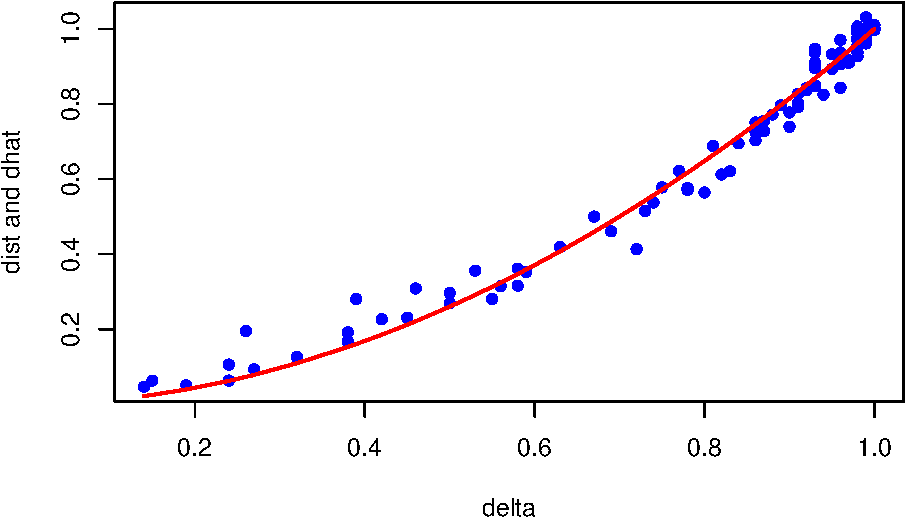
\includegraphics{smacofPO_files/figure-latex/ekman-1.pdf}

Convergence in 24 iterations to stress 0.3002389 and power 1.9421533.

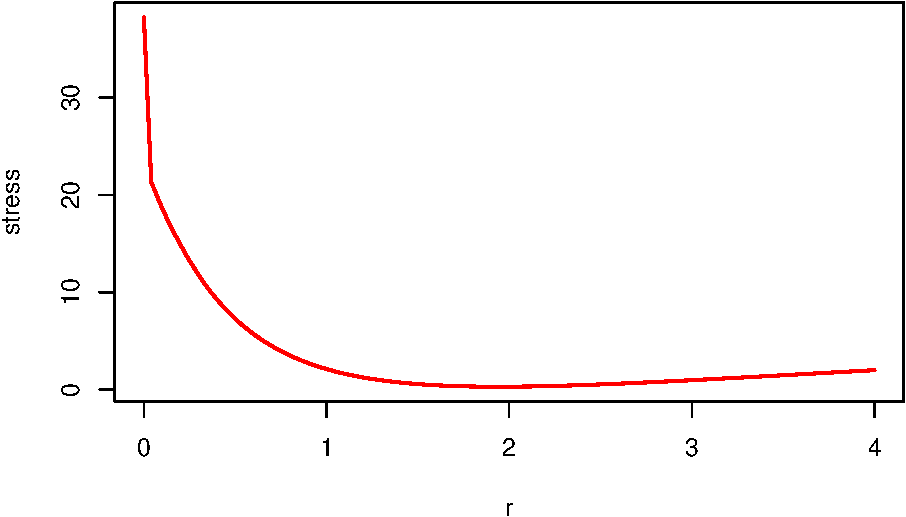
\includegraphics{smacofPO_files/figure-latex/deeper0-1.pdf}

\subsection{De Gruijter (1967)}\label{degruijter_67}

\begin{Shaded}
\begin{Highlighting}[]
\NormalTok{hzero }\OtherTok{\textless{}{-}} \FunctionTok{smacofPO}\NormalTok{(}\DecValTok{1} \SpecialCharTok{{-}} \FunctionTok{diag}\NormalTok{(}\DecValTok{9}\NormalTok{), }\AttributeTok{interval =} \FunctionTok{c}\NormalTok{(}\DecValTok{0}\NormalTok{, }\DecValTok{0}\NormalTok{), }\AttributeTok{eps =} \FloatTok{1e{-}15}\NormalTok{, }\AttributeTok{itmax =} \DecValTok{10000}\NormalTok{, }\AttributeTok{verbose =} \ConstantTok{FALSE}\NormalTok{)}
\end{Highlighting}
\end{Shaded}

Stress at \(r=0\) is 2074.22 and the right derivative of the marginal function at zero is 13.1124395. The largest \(\delta_{ij}\) is 8.13 and the smallest 3.2.

0.5125615

\subsubsection{One}\label{one}

\begin{verbatim}
## [1] -Inf
\end{verbatim}

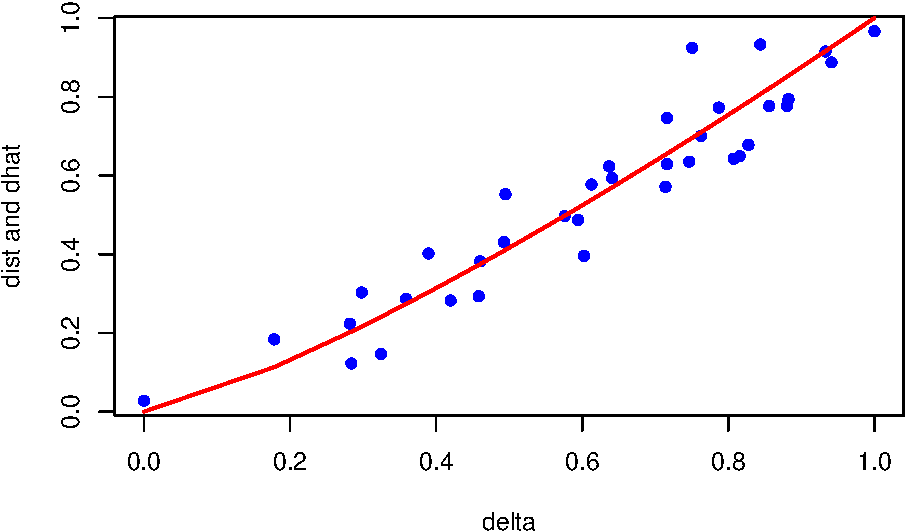
\includegraphics{smacofPO_files/figure-latex/ggruijter-1.pdf}

Convergence in 247 iterations to stress 0.4715325 and power 1.2644972.

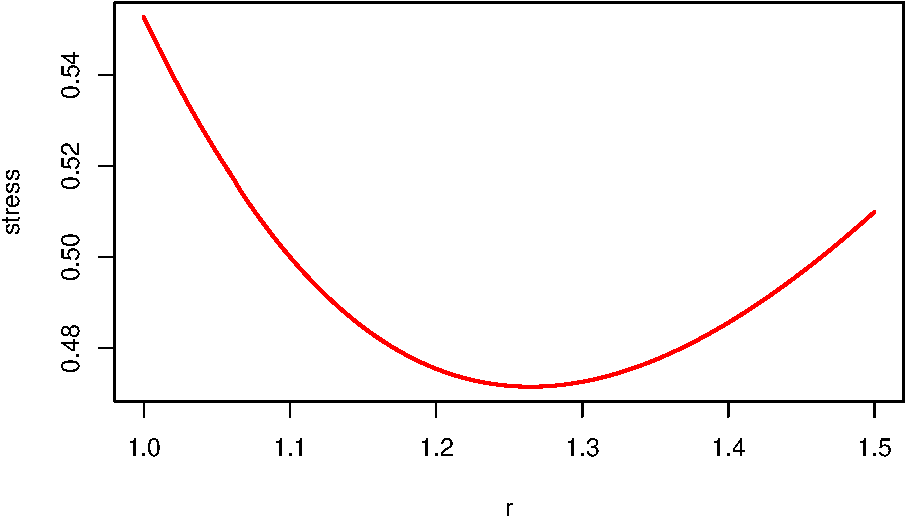
\includegraphics{smacofPO_files/figure-latex/godeeper-1.pdf}

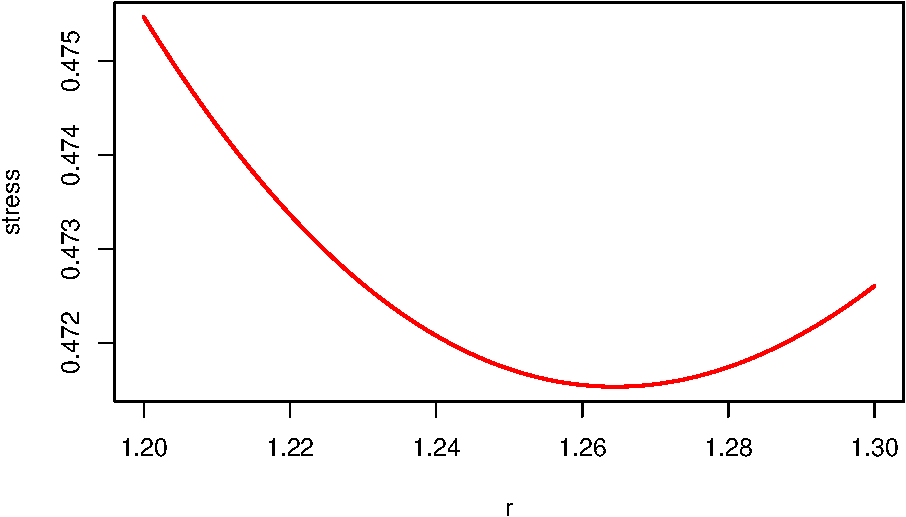
\includegraphics{smacofPO_files/figure-latex/goyetdeeper-1.pdf}

\subsubsection{Two}\label{two}

\begin{verbatim}
## [1] -2.427043
\end{verbatim}

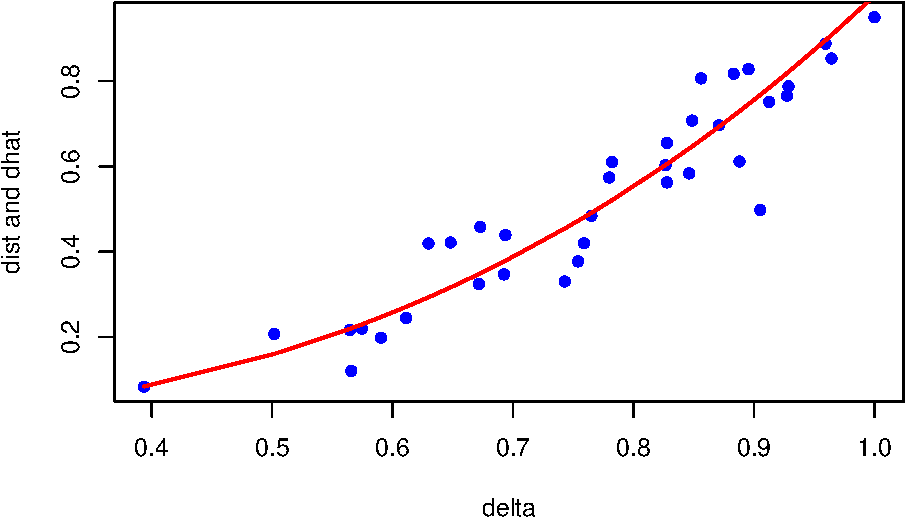
\includegraphics{smacofPO_files/figure-latex/mgruijter-1.pdf}

Convergence in 86 iterations to stress 0.4898419 and power 2.6547464.

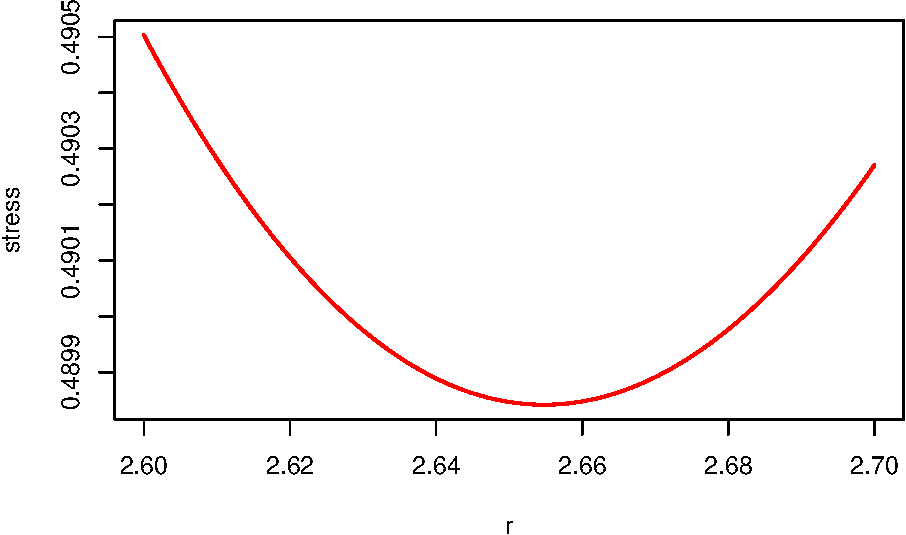
\includegraphics{smacofPO_files/figure-latex/evendeeper-1.pdf}

\subsubsection{Three}\label{three}

\begin{verbatim}
## [1] 13.11244
\end{verbatim}

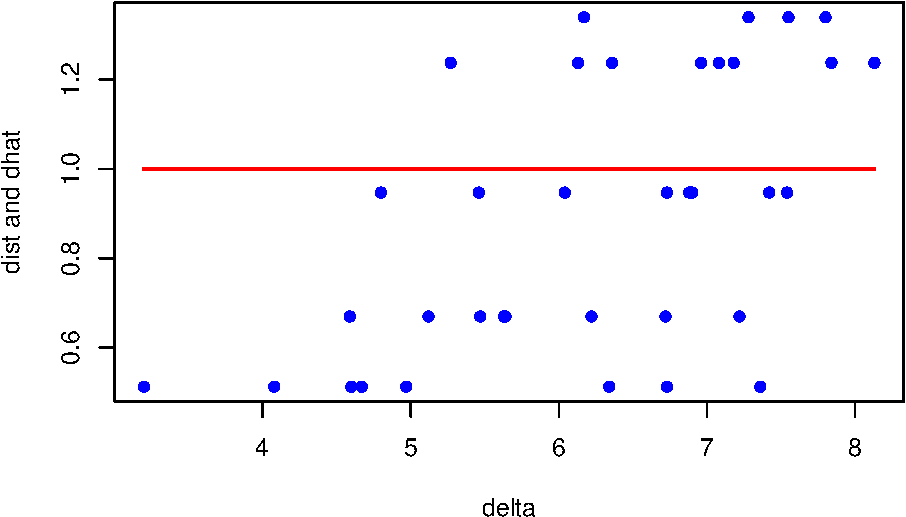
\includegraphics{smacofPO_files/figure-latex/hgruijter-1.pdf}

Convergence in 287 iterations to stress 7.4170928 and power \ensuremath{7.6608779\times 10^{-5}}.

\subsection{Deeper}\label{deeper}

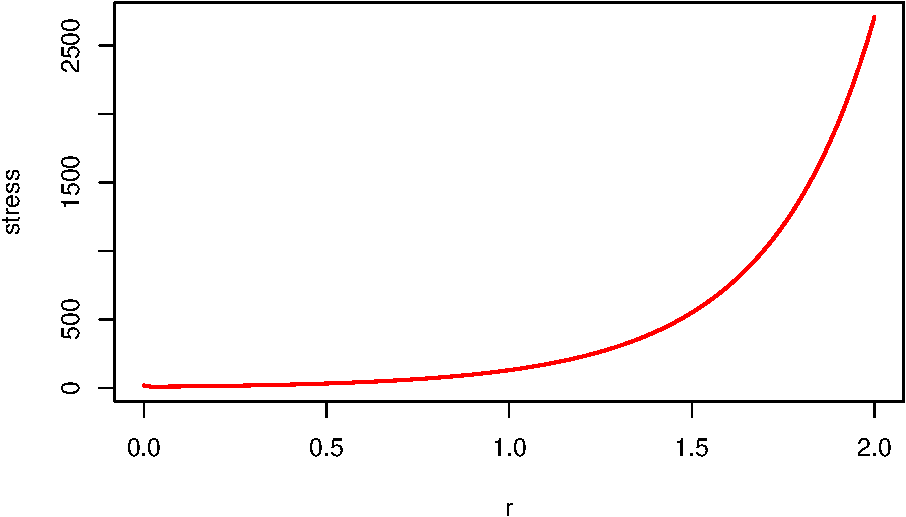
\includegraphics{smacofPO_files/figure-latex/deeper-1.pdf}

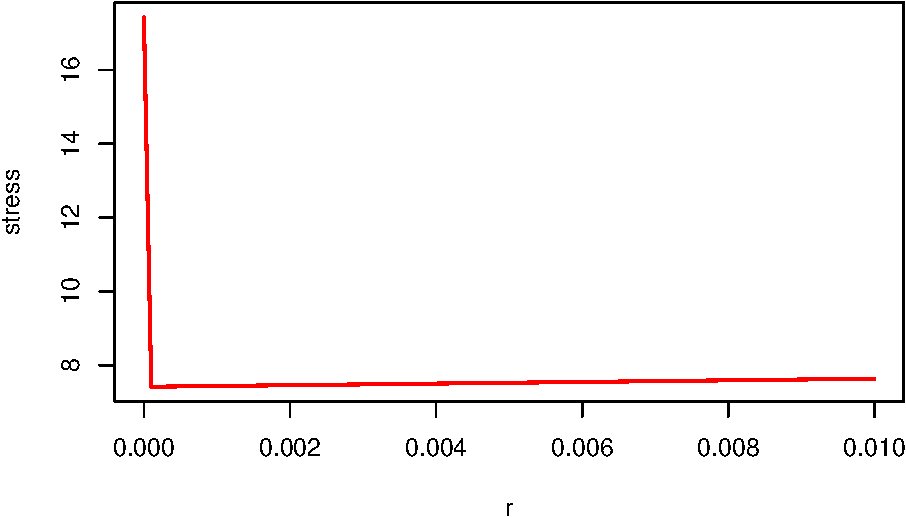
\includegraphics{smacofPO_files/figure-latex/deeper2-1.pdf}

\subsection{Wish (1971)}\label{wish_71}

\begin{Shaded}
\begin{Highlighting}[]
\NormalTok{hzero }\OtherTok{\textless{}{-}} \FunctionTok{smacofPO}\NormalTok{(}\DecValTok{1} \SpecialCharTok{{-}} \FunctionTok{diag}\NormalTok{(}\DecValTok{12}\NormalTok{), }\AttributeTok{interval =} \FunctionTok{c}\NormalTok{(}\DecValTok{0}\NormalTok{, }\DecValTok{0}\NormalTok{), }\AttributeTok{verbose =} \ConstantTok{FALSE}\NormalTok{)}
\end{Highlighting}
\end{Shaded}

Stress at \(r=0\) is 1931.9714 and the right derivative of the marginal function at zero is 25.2469345. The largest \(\delta_{ij}\) is 6.61 and the smallest 2.33.

0.4304788

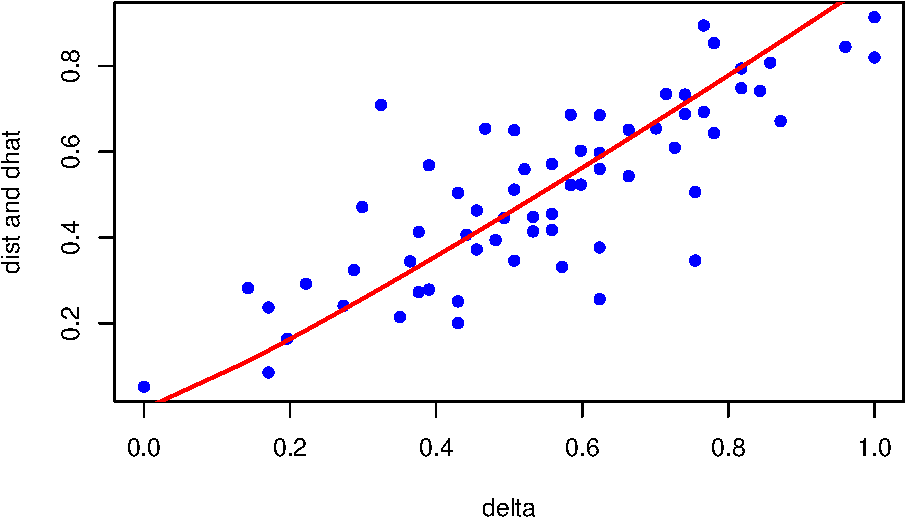
\includegraphics{smacofPO_files/figure-latex/wish-1.pdf}

Convergence in 148 iterations to stress 2.3250238 and power 1.1255951.

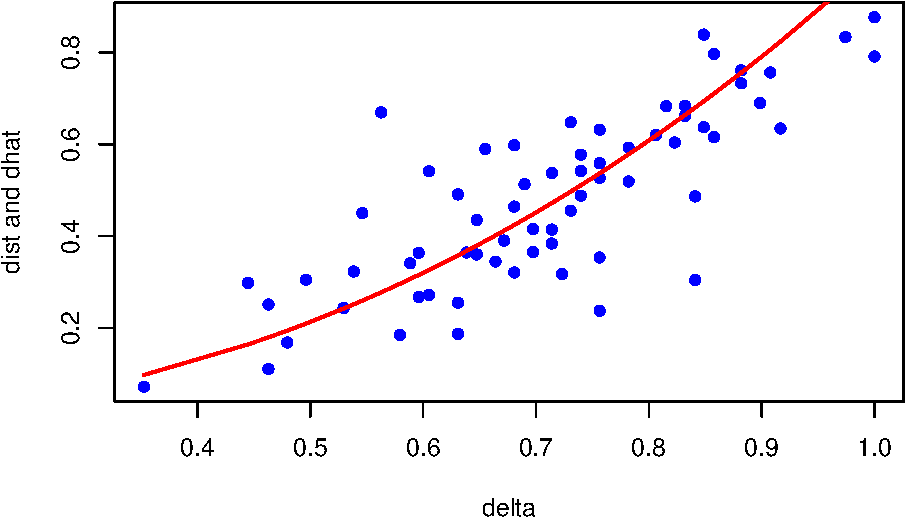
\includegraphics{smacofPO_files/figure-latex/mwish-1.pdf}

Convergence in 166 iterations to stress 2.0296426 and power 2.2292659.

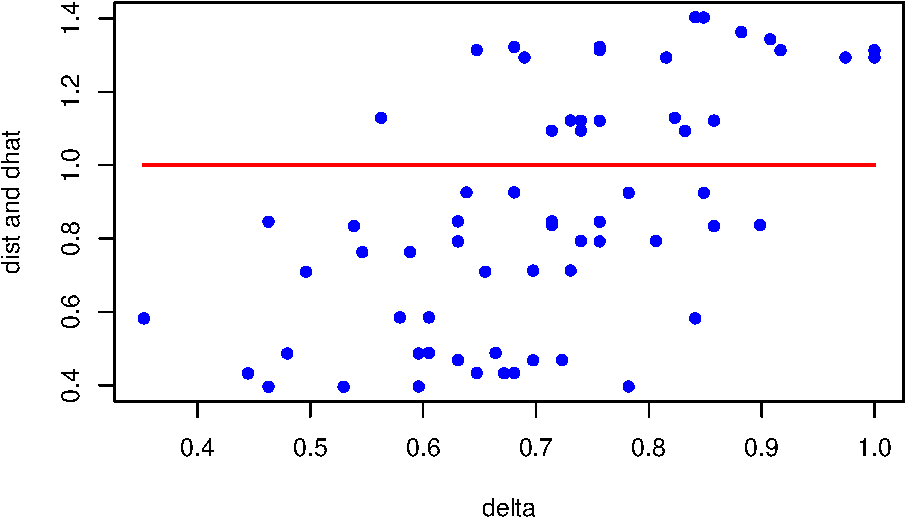
\includegraphics{smacofPO_files/figure-latex/hwish-1.pdf}

Convergence in 2656 iterations to stress 15.9244051 and power \ensuremath{6.4120229\times 10^{-5}}.

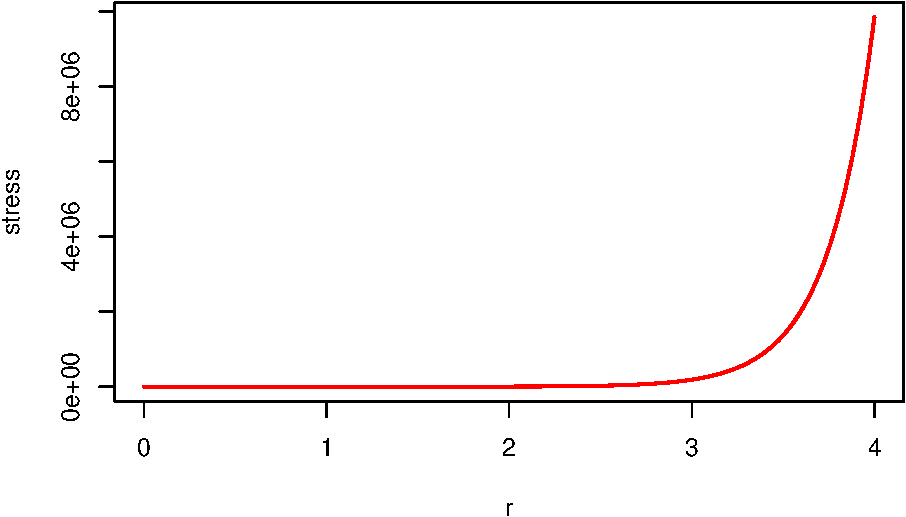
\includegraphics{smacofPO_files/figure-latex/deeper3-1.pdf}

\subsection{Rothkopf (1957)}\label{rothkopf_57}

\begin{Shaded}
\begin{Highlighting}[]
\NormalTok{hzero }\OtherTok{\textless{}{-}} \FunctionTok{smacofPO}\NormalTok{(}\DecValTok{1} \SpecialCharTok{{-}} \FunctionTok{diag}\NormalTok{(}\DecValTok{36}\NormalTok{), }\AttributeTok{xe =} \FunctionTok{matrix}\NormalTok{(}\FunctionTok{rnorm}\NormalTok{(}\DecValTok{72}\NormalTok{), }\DecValTok{36}\NormalTok{, }\DecValTok{2}\NormalTok{), }\AttributeTok{interval =} \FunctionTok{c}\NormalTok{(}\DecValTok{0}\NormalTok{, }\DecValTok{0}\NormalTok{), }\AttributeTok{verbose =} \ConstantTok{FALSE}\NormalTok{, }\AttributeTok{itmax =} \DecValTok{10000}\NormalTok{)}
\NormalTok{hone }\OtherTok{\textless{}{-}} \FunctionTok{smacofPO}\NormalTok{(}\FunctionTok{as.matrix}\NormalTok{(morse), }\AttributeTok{xe =} \ConstantTok{NULL}\NormalTok{, }\AttributeTok{interval =} \FunctionTok{c}\NormalTok{(}\DecValTok{1}\NormalTok{, }\DecValTok{1}\NormalTok{), }\AttributeTok{verbose =} \ConstantTok{FALSE}\NormalTok{, }\AttributeTok{itmax =} \DecValTok{10000}\NormalTok{)}
\end{Highlighting}
\end{Shaded}

Stress at \(r=0\) is 104.2792 and the right derivative of the marginal function at zero is -47.7485475. The largest \(\delta_{ij}\) is 0.98 and the smallest 0.2. Stress at \(r=1\) is 80.3674371.

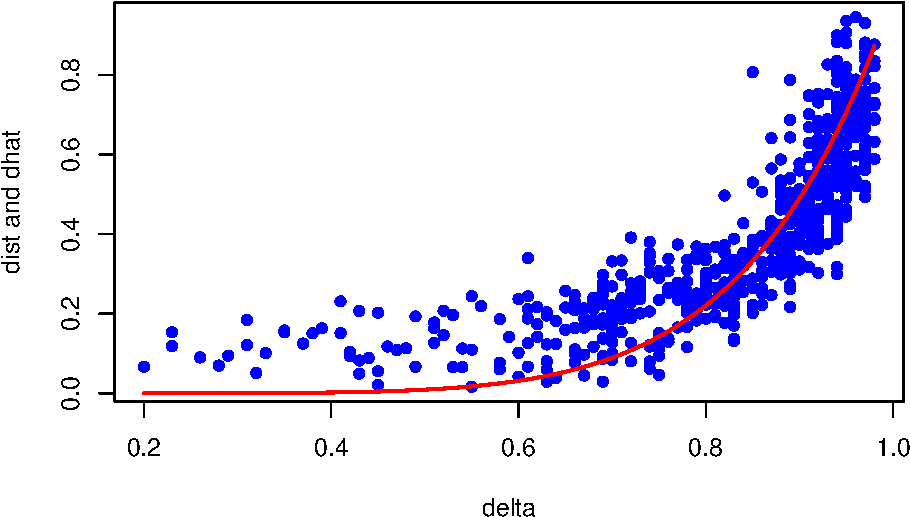
\includegraphics{smacofPO_files/figure-latex/morse-1.pdf}

Convergence in 253 iterations to stress 18.5193005 and power 6.7735801.

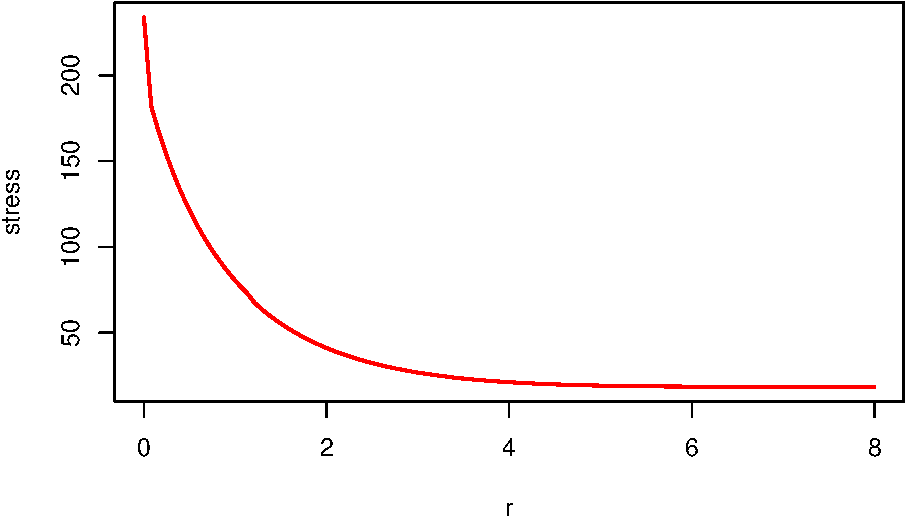
\includegraphics{smacofPO_files/figure-latex/deeper5-1.pdf}

\section{Code}\label{code}

\begin{Shaded}
\begin{Highlighting}[]
\NormalTok{smacofPO }\OtherTok{\textless{}{-}}
  \ControlFlowTok{function}\NormalTok{(delta,}
           \AttributeTok{interval =} \FunctionTok{c}\NormalTok{(}\DecValTok{0}\NormalTok{, }\DecValTok{4}\NormalTok{),}
           \AttributeTok{xold =} \ConstantTok{NULL}\NormalTok{,}
           \AttributeTok{itmax =} \DecValTok{1000}\NormalTok{,}
           \AttributeTok{eps =} \FloatTok{1e{-}10}\NormalTok{,}
           \AttributeTok{verbose =} \ConstantTok{TRUE}\NormalTok{) \{}
\NormalTok{    nobj }\OtherTok{\textless{}{-}} \FunctionTok{nrow}\NormalTok{(delta)}
\NormalTok{    dd }\OtherTok{\textless{}{-}}\NormalTok{ delta }\SpecialCharTok{\^{}} \DecValTok{2}
\NormalTok{    rd }\OtherTok{\textless{}{-}} \FunctionTok{rowSums}\NormalTok{(dd) }\SpecialCharTok{/}\NormalTok{ nobj}
\NormalTok{    sd }\OtherTok{\textless{}{-}} \FunctionTok{mean}\NormalTok{(delta)}
\NormalTok{    ce }\OtherTok{\textless{}{-}} \SpecialCharTok{{-}}\NormalTok{.}\DecValTok{5} \SpecialCharTok{*}\NormalTok{ (dd }\SpecialCharTok{{-}} \FunctionTok{outer}\NormalTok{(rd, rd) }\SpecialCharTok{+}\NormalTok{ sd)}
\NormalTok{    ee }\OtherTok{\textless{}{-}} \FunctionTok{eigen}\NormalTok{(ce)}
\NormalTok{    xe }\OtherTok{\textless{}{-}}\NormalTok{ ee}\SpecialCharTok{$}\NormalTok{vectors[, }\DecValTok{1}\SpecialCharTok{:}\DecValTok{2}\NormalTok{] }\SpecialCharTok{\%*\%} \FunctionTok{diag}\NormalTok{(}\FunctionTok{sqrt}\NormalTok{(ee}\SpecialCharTok{$}\NormalTok{values[}\DecValTok{1}\SpecialCharTok{:}\DecValTok{2}\NormalTok{]))}
\NormalTok{    de }\OtherTok{\textless{}{-}} \FunctionTok{as.matrix}\NormalTok{(}\FunctionTok{dist}\NormalTok{(xe))}
    \ControlFlowTok{if}\NormalTok{ (interval[}\DecValTok{1}\NormalTok{] }\SpecialCharTok{==}\NormalTok{ interval[}\DecValTok{2}\NormalTok{]) \{}
\NormalTok{      r }\OtherTok{\textless{}{-}}\NormalTok{ interval[}\DecValTok{1}\NormalTok{]}
\NormalTok{      fixed }\OtherTok{\textless{}{-}} \ConstantTok{TRUE}
\NormalTok{    \} }\ControlFlowTok{else}\NormalTok{ \{}
\NormalTok{      r }\OtherTok{\textless{}{-}}\NormalTok{ (interval[}\DecValTok{1}\NormalTok{] }\SpecialCharTok{+}\NormalTok{ interval[}\DecValTok{2}\NormalTok{]) }\SpecialCharTok{/} \DecValTok{2}
\NormalTok{    \}}
\NormalTok{    g }\OtherTok{\textless{}{-}} \ControlFlowTok{function}\NormalTok{(r, delta, de) \{}
      \FunctionTok{return}\NormalTok{(}\FunctionTok{sum}\NormalTok{(((delta }\SpecialCharTok{\^{}}\NormalTok{ r) }\SpecialCharTok{{-}}\NormalTok{ de) }\SpecialCharTok{\^{}} \DecValTok{2}\NormalTok{))}
\NormalTok{    \}}
\NormalTok{    ep }\OtherTok{\textless{}{-}}\NormalTok{ delta }\SpecialCharTok{\^{}}\NormalTok{ r}
\NormalTok{    sold }\OtherTok{\textless{}{-}} \FunctionTok{sum}\NormalTok{((ep }\SpecialCharTok{{-}}\NormalTok{ de) }\SpecialCharTok{\^{}} \DecValTok{2}\NormalTok{)}
\NormalTok{    itel }\OtherTok{\textless{}{-}} \DecValTok{1}
    \ControlFlowTok{repeat}\NormalTok{ \{}
\NormalTok{      b }\OtherTok{\textless{}{-}} \SpecialCharTok{{-}}\NormalTok{ep }\SpecialCharTok{/}\NormalTok{ (de }\SpecialCharTok{+} \FunctionTok{diag}\NormalTok{(nobj))}
      \FunctionTok{diag}\NormalTok{(b) }\OtherTok{\textless{}{-}} \SpecialCharTok{{-}}\FunctionTok{rowSums}\NormalTok{(b)}
\NormalTok{      xe }\OtherTok{\textless{}{-}}\NormalTok{ (b }\SpecialCharTok{\%*\%}\NormalTok{ xe) }\SpecialCharTok{/}\NormalTok{ nobj}
\NormalTok{      de }\OtherTok{\textless{}{-}} \FunctionTok{as.matrix}\NormalTok{(}\FunctionTok{dist}\NormalTok{(xe))}
\NormalTok{      smid }\OtherTok{\textless{}{-}} \FunctionTok{sum}\NormalTok{((ep }\SpecialCharTok{{-}}\NormalTok{ de) }\SpecialCharTok{\^{}} \DecValTok{2}\NormalTok{)}
      \ControlFlowTok{if}\NormalTok{ (}\SpecialCharTok{!}\NormalTok{fixed) \{}
\NormalTok{        r }\OtherTok{\textless{}{-}} \FunctionTok{optimize}\NormalTok{(g, }\AttributeTok{interval =}\NormalTok{ interval, }\AttributeTok{delta =}\NormalTok{ delta, }\AttributeTok{de =}\NormalTok{ de)}\SpecialCharTok{$}\NormalTok{minimum}
\NormalTok{      \}}
\NormalTok{      ep }\OtherTok{\textless{}{-}}\NormalTok{ delta }\SpecialCharTok{\^{}}\NormalTok{ r}
\NormalTok{      snew }\OtherTok{\textless{}{-}} \FunctionTok{sum}\NormalTok{((ep }\SpecialCharTok{{-}}\NormalTok{ de) }\SpecialCharTok{\^{}} \DecValTok{2}\NormalTok{)}
      \ControlFlowTok{if}\NormalTok{ (verbose) \{}
        \FunctionTok{cat}\NormalTok{(}
          \StringTok{"itel "}\NormalTok{,}
          \FunctionTok{formatC}\NormalTok{(itel, }\AttributeTok{format =} \StringTok{"d"}\NormalTok{),}
          \StringTok{"sold "}\NormalTok{,}
          \FunctionTok{formatC}\NormalTok{(sold, }\AttributeTok{digits =} \DecValTok{6}\NormalTok{, }\AttributeTok{format =} \StringTok{"f"}\NormalTok{),}
          \StringTok{"smid "}\NormalTok{,}
          \FunctionTok{formatC}\NormalTok{(smid, }\AttributeTok{digits =} \DecValTok{6}\NormalTok{, }\AttributeTok{format =} \StringTok{"f"}\NormalTok{),}
          \StringTok{"snew "}\NormalTok{,}
          \FunctionTok{formatC}\NormalTok{(snew, }\AttributeTok{digits =} \DecValTok{6}\NormalTok{, }\AttributeTok{format =} \StringTok{"f"}\NormalTok{),}
          \StringTok{"pow  "}\NormalTok{,}
          \FunctionTok{formatC}\NormalTok{(r, }\AttributeTok{digits =} \DecValTok{6}\NormalTok{, }\AttributeTok{format =} \StringTok{"f"}\NormalTok{),}
          \StringTok{"}\SpecialCharTok{\textbackslash{}n}\StringTok{"}
\NormalTok{        )}
\NormalTok{      \}}
      \ControlFlowTok{if}\NormalTok{ (((sold }\SpecialCharTok{{-}}\NormalTok{ snew) }\SpecialCharTok{\textless{}} \FloatTok{1e{-}10}\NormalTok{) }\SpecialCharTok{||}\NormalTok{ (itel }\SpecialCharTok{==}\NormalTok{ itmax)) \{}
        \ControlFlowTok{break}
\NormalTok{      \}}
\NormalTok{      itel }\OtherTok{\textless{}{-}}\NormalTok{ itel }\SpecialCharTok{+} \DecValTok{1}
\NormalTok{      sold }\OtherTok{\textless{}{-}}\NormalTok{ snew}
\NormalTok{    \}}
    \FunctionTok{return}\NormalTok{(}\FunctionTok{list}\NormalTok{(}
      \AttributeTok{x =}\NormalTok{ xe,}
      \AttributeTok{d =}\NormalTok{ de,}
      \AttributeTok{e =}\NormalTok{ ep,}
      \AttributeTok{r =}\NormalTok{ r,}
      \AttributeTok{itel =}\NormalTok{ itel,}
      \AttributeTok{stress =}\NormalTok{ snew}
\NormalTok{    ))}
\NormalTok{  \}}
\end{Highlighting}
\end{Shaded}

\phantomsection\label{refs}
\begin{CSLReferences}{1}{0}
\bibitem[\citeproctext]{ref-degruijter_67}
De Gruijter, D. N. M. 1967. {``{The Cognitive Structure of Dutch Political Parties in 1966}.''} Report E019-67. Psychological Institute, University of Leiden.

\bibitem[\citeproctext]{ref-deleeuw_U_14c}
De Leeuw, J. 2014. {``{Minimizing rStress Using Nested Majorization}.''} UCLA Department of Statistics. \url{https://jansweb.netlify.app/publication/deleeuw-u-14-c/deleeuw-u-14-c.pdf}.

\bibitem[\citeproctext]{ref-deleeuw_groenen_mair_E_16h}
De Leeuw, J., P. Groenen, and P. Mair. 2016a. {``Minimizing qStress for Small q.''} 2016. \url{https://jansweb.netlify.app/publication/deleeuw-groenen-mair-e-16-h/deleeuw-groenen-mair-e-16-h.pdf}.

\bibitem[\citeproctext]{ref-deleeuw_groenen_mair_E_16a}
---------. 2016b. {``{Minimizing rStress Using Majorization}.''} 2016. \url{https://jansweb.netlify.app/publication/deleeuw-groenen-mair-e-16-a/deleeuw-groenen-mair-e-16-a.pdf}.

\bibitem[\citeproctext]{ref-deleeuw_stoop_A_84}
De Leeuw, J., and I. Stoop. 1984. {``Upper Bounds for Kruskal's Stress.''} \emph{Psychometrika} 49: 391--402.

\bibitem[\citeproctext]{ref-ekman_54}
Ekman, G. 1954. {``{Dimensions of Color Vision}.''} \emph{Journal of Psychology} 38: 467--74.

\bibitem[\citeproctext]{ref-groenen_deleeuw_U_10}
Groenen, P. J. F., and J. De Leeuw. 2010. {``{Power-Stress for Multidimensional Scaling}.''} \url{https://jansweb.netlify.app/publication/groenen-deleeuw-u-10/groenen-deleeuw-u-10.pdf}.

\bibitem[\citeproctext]{ref-guttman_68}
Guttman, L. 1968. {``{A General Nonmetric Technique for Fitting the Smallest Coordinate Space for a Configuration of Points}.''} \emph{Psychometrika} 33: 469--506.

\bibitem[\citeproctext]{ref-kruskal_64a}
Kruskal, J. B. 1964. {``{Multidimensional Scaling by Optimizing Goodness of Fit to a Nonmetric Hypothesis}.''} \emph{Psychometrika} 29: 1--27.

\bibitem[\citeproctext]{ref-luce_59}
Luce, R. D. 1959. {``On the Possible Psychophysical Laws.''} \emph{Psychologicsal Review} 66 (2): 81--95.

\bibitem[\citeproctext]{ref-rothkopf_57}
Rothkopf, E. Z. 1957. {``{A Measure of Stimulus Similarity and Errors in some Paired-associate Learning}.''} \emph{Journal of Experimental Psychology} 53: 94--101.

\bibitem[\citeproctext]{ref-stevens_57}
Stevens, S. S. 1957. {``On the Psychophysical Law.''} \emph{Psychological Review} 64 (3): 153--81.

\bibitem[\citeproctext]{ref-wish_71}
Wish, M. 1971. {``Individual Differences in Perceptions and Preferences Among Nations.''} In \emph{Attitude Research Reaches New Heights}, edited by C. W. King and D. Tigert, 312--28. American Marketing Association.

\end{CSLReferences}

\end{document}
